\section{Motivation and Background}
\label{sec:background}

Over the last decade single GPU performance has scaled thanks to a 
significant growth in per-GPU transistor count and DRAM bandwidth. For 
example, in 2010 NVIDIA's Fermi GPU integrated 1.95B transistors on a 
529mm\textsuperscript{2} die, with 180GB/s of DRAM 
bandwidth~\cite{hennessypatterson11}. In 2016 NVIDIA's Pascal GPU 
contained 12B transistors within a 610 mm\textsuperscript{2} die, while 
relying on 720GB/s of memory bandwidth~\cite{inside-pascal}. Unfortunately, 
transistor density is slowing significantly and many integrated circuit 
manufacturers are not providing roadmaps beyond 7nm. Moreover, GPU die sizes,
which have been also slowly but steadily growing generationally, are 
expected to slow down due to limitations in lithography and manufacturing cost.

\begin{figure}[t] 
    \centering
    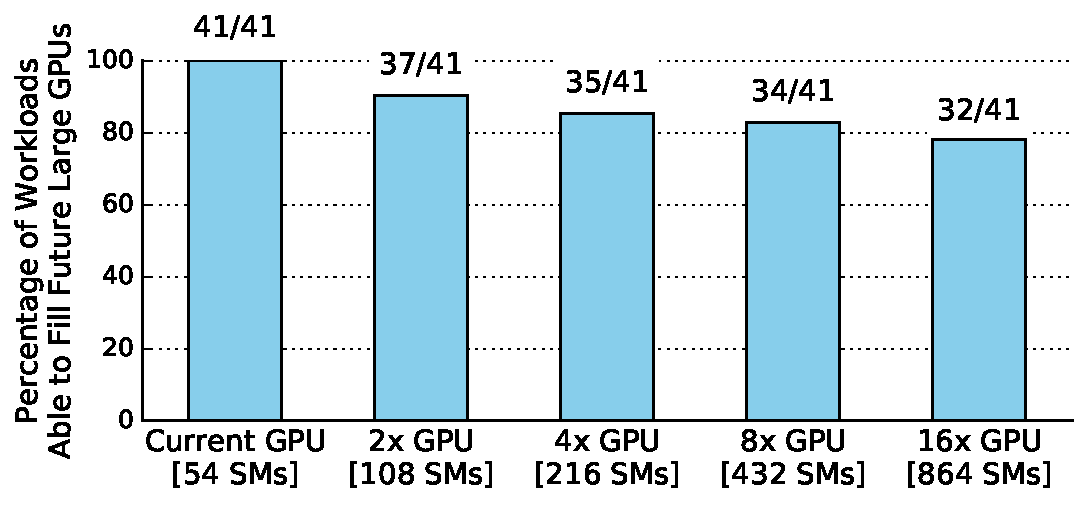
\includegraphics[width=1.0\columnwidth]{figures/plot_ctas_per_sm.pdf}
    \caption{Percentage of workloads that are able to fill future larger GPUs 
    (average number of concurrent thread blocks exceeds number of SMs in the system).}
    \label{fig:ctas}
    \vspace{-.2in}
\end{figure}

Without either larger or denser dies, GPU architects must turn to 
alternative solutions to significantly increase GPU performance.  Recently 3D 
die-stacking has seen significant interest due to its successes with high 
bandwidth DRAM~\cite{HBM}. Unfortunately 3D die-stacking still has 
a significant engineering challenges related to power delivery, 
energy density, and cooling~\cite{verbree2010cost} when employed in power 
hungry, maximal die-sized chips such as GPUs. Thus we propose GPU manufacturers 
are likely to re-examine a tried and trued solution from CPU world, 
\textit{multi-socket GPUs}, to scaling GPU performance while maintaining the 
current ratio of floating point operations per second (FLOPS) and DRAM 
bandwidth.

Multi-socket GPUs are enabled by the evolution of GPUs from external
peripherals to central computing components, considered at system design time.  
GPU optimized systems now employ custom PCB designs that accommodate 
high pin count socketed GPUs~\cite{dgx} with inter-GPU interconnects resembling 
QPI or HyperTransport~\cite{NVLINK,INTELQPI,AMDHT}.  Despite the rapid 
improvement in hardware capabilities, these systems have 
continued to expose the GPUs provided as individually addressable units. These
multi-GPU systems can provide high aggregate throughput when running multiple concurrent
GPU kernels, but to accelerate a single GPU workload they
require layering additional software runtimes on top of native GPU programming 
interfaces such as CUDA or openCL~\cite{CUDA,OPENCL}. Unfortunately, by requiring
application re-design many workloads are never ported to take advantage
of multiple GPUs.

Extending single GPU workload performance significantly is a laudable
goal, but we must first understand if these applications will be able to leverage
larger GPUs.  Today NVIDIA's largest GPUs contain 56 SMs; across a benchmark set of 41 applications
(later described in Section~\ref{sec:methodology}),
Figure~\ref{fig:ctas} shows that most single GPU optimized workloads already
contain sufficient data parallelism to fill GPUs that are 2--8$\times$ larger 
than today's biggest GPUs.  While these applications are unlikely to ever scale to tens
of thousands of GPUs across an entire data center, we believe that programmer
transparent workload scaling (up to 8$\times$) will
be attractive to many GPU developers.

In this work, we examine the performance of a future 4-socket NUMA GPU to 
understand the effects that NUMA will have when executing applications designed 
for UMA GPUs. We will show (not surprisingly), that when executing UMA-optimized 
GPU programs on a multi-socket NUMA GPU, performance does not scale.  We draw on 
prior work and show that before optimizing GPU microarchitecture for 
NUMA-awareness, several software optimizations must be in place to preserve data 
locality.  Alone these SW improvements are not sufficient to achieve scalable 
performance however and interconnect bandwidth is a significant hindrance on 
performance.  To overcome this bottleneck we propose two classes of improvements 
to reduce the observed NUMA penalty.

First, in Section~\ref{sec:interconnect} we examine the 
ability of switch connected GPUs to dynamically repartition their ingress and 
egress links to provide asymmetric bandwidth provisioning when required.  By 
using existing interconnects more efficiently the effective NUMA bandwidth ratio 
of remote memory to local memory decreases, improving performance. Second, 
to minimize traffic on oversubscribed interconnect links we propose GPU caches need 
to become NUMA-aware in Section~\ref{sec:caches}. Traditional on-chip caches are 
optimized to maximize 
overall hitrate, thus minimizing off-chip bandwidth, However, in NUMA 
systems, not all cache misses have the same relative cost and thus should not 
be treated equally. Due to the NUMA penalty of accessing remote memory, we show 
that performance can be maximized by preferencing cache capacity (and thus 
improving hit rate) towards data that resides in slower remote NUMA zones, at the 
expense of data that resides in faster local NUMA zones. To this end, we propose 
a new NUMA-aware cache architecture that dynamically balances cache capacity based on 
memory system utilization. Before diving into microarchitectural details and results,
we first describe the locality optimized GPU SW runtime that enables our proposed
NUMA-aware architecture.

\begin{figure*}[tp] 
    \centering
    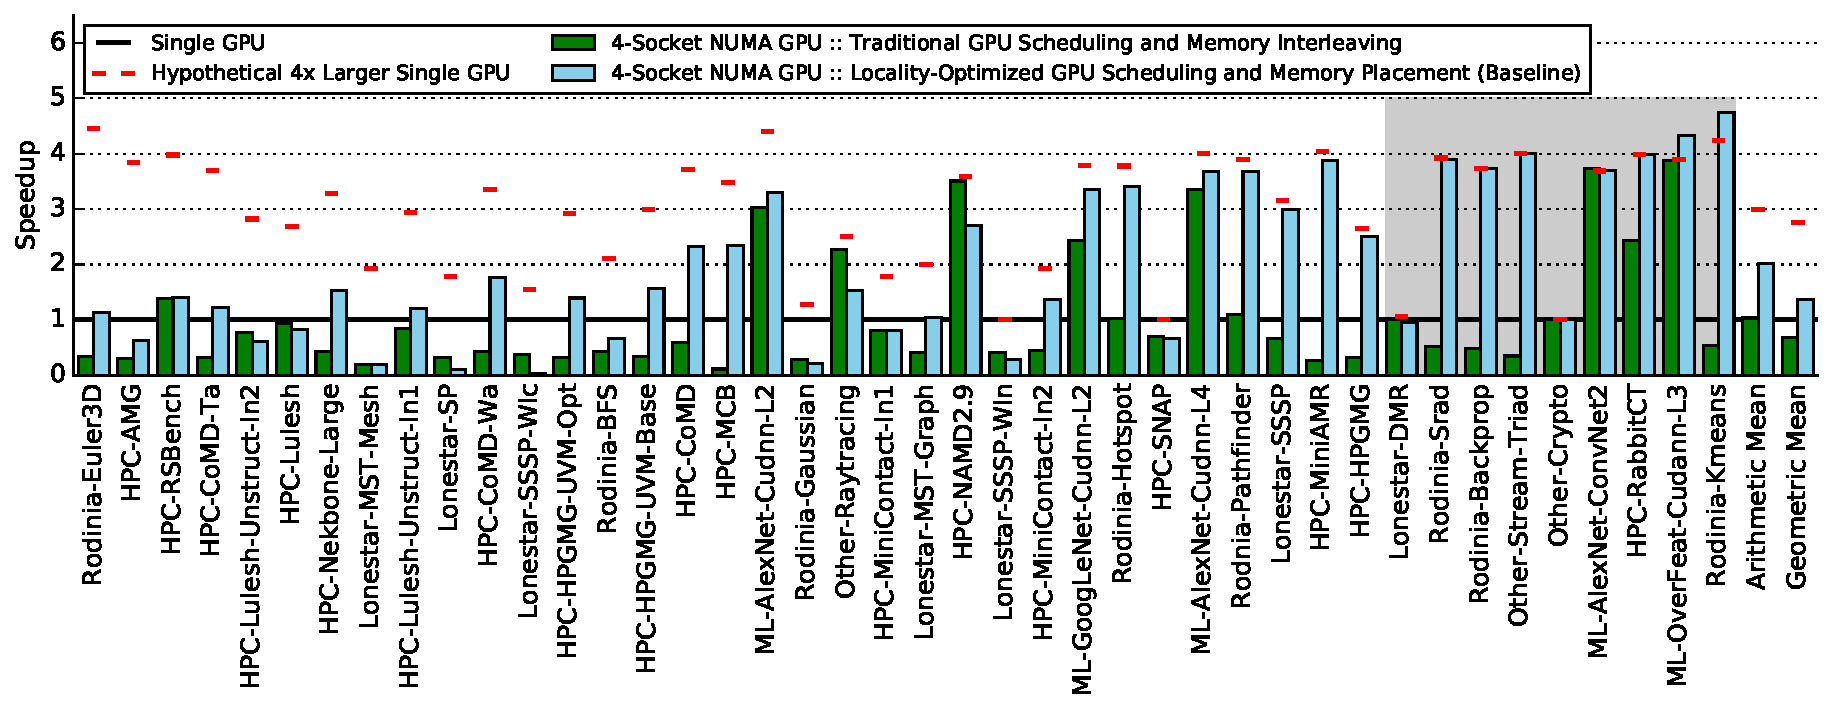
\includegraphics[width=1.0\linewidth]{figures/plot_different_baselines.pdf}
    \caption{Relative performance of a 4-socket NUMA GPU using to a single GPU 
and a hypothetical 4$\times$ larger (all resources scaled) single GPU showing 
upper bound of performance this application can achieve via GPU hardware 
scaling. For the Locality-Optimized design, applications shown in grey 
achieve already 99\% of theoretical scaling (\emph{red dash}) without 
micro-architectural modification.}
    \label{fig:motivation}
    \vspace{-.2in}
\end{figure*}
